\documentclass{beamer}

% theme definition
\usetheme{KU}

\usepackage{natbib}
\usepackage{alltt}
\usepackage{trust}

\setbeamertemplate{blocks}[rounded][shadow=true]

\setbeamercolor{title}{fg=kublue}
\setbeamercolor{subtitle}{fg=kugray} 
\setbeamercolor{institute}{fg=kugray}
\setbeamercolor{frametitle}{fg=kublue}
\setbeamercolor{frametitle}{bg=white}
\setbeamercolor{framesubtitle}{fg=kugray}
\setbeamercolor{framesubtitle}{bg=white}
\setbeamercolor{item}{fg=black}
\setbeamercolor{subitem}{fg=kugray}
\setbeamercolor{itemize/enumerate subbody}{fg=kugray}
\setbeamercolor{block title}{bg=kublue}
\setbeamercolor{block title}{fg=white}
\setbeamercolor{block body}{bg=sand}
\setbeamercolor{block body}{fg=black}

\usefonttheme{serif}

\newenvironment{fnverbatim}{\begin{alltt}\scriptsize}{\normalsize\end{alltt}}
\newcommand{\mean}[1]{\langle#1\rangle}
\newcommand{\rtime}{\ensuremath{\mathbb{R}^{0\leq}}}

\bibliographystyle{abbrv}

\title{Trust}
\subtitle{What it is and how to get it}

\author{Dr. Perry Alexander}

%\date{{\color{kugray}\today}}
\date{\ }

% turns off navigation symbols
\setbeamertemplate{navigation symbols}{}

\institute{
    Information and Telecommunication Technology Center \\
    Electrical Engineering and Computer Science \\
    The University of Kansas \\
    \texttt{palexand@ku.edu}}

\begin{document}

\begin{frame}
  \titlepage

{\footnotesize\color{kugray} Formatted with the KU Beamer Class for \LaTeXe}
\end{frame}

\frame{\frametitle{What is Trust?}
  ``An entity can be trusted if it always behaves in the expected
  manner for the intended purpose''\footnote{\emph{The Ten Page Introduction
      to Trusted Computing} by Andrew Martin}
}

\frame{\frametitle{Properties of Trust}
    \begin{itemize}
    \item Unambiguous identification
    \item Unimpeded operation
    \item First-hand observation of good behavior \emph{or} indirect
      experience of good behavior by a trusted third party
    \end{itemize}
}

\frame{\frametitle{Required Capabilities for Establishing Trust}
  \begin{itemize}
  \item \emph{Strong Identification} --- An unambiguous, immutable
    identifier associated with the platform.
  \item \emph{Reporting Configuration} --- An unambiguous
    identification mechanism for software and hardware running on the
    platform.
  \item \emph{Reporting Behavior} --- A mechanism for observing and reporting execution behavior.
  \end{itemize}
}

\frame{\frametitle{Tools for Trust}
  \begin{itemize}
  \item $\hash{X}$ --- Hash of $X$
    \begin{itemize}
    \item $\hash{X}$ is unique for each $X$
    \item Guessing $X$ from $\hash{X}$ is impossible
    \end{itemize}
  \item $\encrypt{X}{Y}$ --- Encrypt $X$ with $\public{Y}$
    \begin{itemize}
    \item $X$ cannot be obtained from $\encrypt{X}{Y}$ without $Y$
    \item Guessing $X$ from $\encrypt{X}{Y}$ is impossible
    \item Guessing $Y$ is impossible
    \end{itemize}
  \item $\sign{X}{Y}$ --- Sign $X$ with $\private{Y}$
    \begin{itemize}
    \item $\sign{X}{Y}$ is unique for every $X$ and $\private{Y}$ pair
    \item Guessing $\sign{X}{Y}$ from $X$ is impossible
    \end{itemize}
  \item $\extend{M}{\hash{X}}$ --- Extend $M$ with $\hash{X}$
    \begin{itemize}
    \item Concatenate $M$ with $\hash{X}$ and hash the result
    \item Ideal $\extend{M}{\hash{X}}$ unique for $M$ and $X$	
    \end{itemize}
  \end{itemize}
}

\frame{\frametitle{Tools for Trust}
  \begin{itemize}
  \item $\wrap{X}{\private{Y}}$ --- Wrap $X$ with $\private{Y}$
    \begin{itemize}
    \item Can use $\public{X}$ for encryption and signature checking
    \item Cannot use $\private{X}$ for decryption or signing without $\private{Y}$
    \end{itemize}
  \item $\seal{D}{C}$ --- Seal $D$ to configuration $C$
    \begin{itemize}
    \item $D$ is not available if system is not in configuration $C$
    \item Usually accompanied by encryption
    \end{itemize}
  \item $\envelope{\public{K}}{D}$ --- Envelope $D$ with $\public{K}$
    \begin{itemize}
    \item Encrypt large data $D$ with session key $SK$
    \item Encrypt $SK$ with $\public{K}$
    \item $D$ behaves as if encrypted with $\public{K}$
    \end{itemize}
  \item $\cert{(A,B)}{\private{Y}}$ --- Certify binding of $A$ and $B$ with $\private{Y}$ 
    \begin{itemize}
    \item $Y$ signs $(A,B)$ with private key $\private{Y}$
    \item Certificate is checked using $\public{Y}$
    \item Valid signature provides evidence $A$ and $B$ are bound together
    \end{itemize}
  \end{itemize}
}

\frame{\frametitle{Wrapping and Chaining Keys}
  
  \begin{block}{Wrapping A Key}
    $wrap(X,Y) = \wrap{X}{\private{Y}}$
  \end{block}

  \begin{itemize}
  \item $\private{X}$ is encrypted with $\private{Y}$ while
    $\public{X}$ is clear 
  \item $\encrypt{D}{X}$ and checking $\sign{D}{X}$ may be done
    without $Y$
  \item Decrypting $\encrypt{D}{X}$ and generating $\sign{D}{X}$
    require $Y$
  \end{itemize}
  
  \begin{block}{Chaining Keys}
    $\wrap{X_0}{\private{X_1}}$,$\wrap{X_1}{\private{X_2}}$ $\ldots$
    $\wrap{X_{n-1}}{\private{X_n}}$
  \end{block}

  \begin{itemize}
  \item Each key depends on the previous key
  \item If the root key is trustworthy the chain is trustworthy
  \end{itemize}

}

\frame{\frametitle{Installing Keys}

  \begin{block}{Wrapped Keys}
      A wrapped key must be installed before use and depends on
      installation of its wrapping key
  \end{block}
  

  \begin{itemize}
  \item Installing $\wrap{K}{\private{J}}$ provides a handle for use with
    other commands
    \begin{itemize}
    \item The key handle is a pointer into the TPM
    \item Cannot be used to access the key outside the TPM
    \end{itemize}
  \item $\wrap{K}{\private{J}}$ installs if $\public{J}$ is installed
    and usable
    \begin{itemize}
    \item Key may be installed by not usable if PCRs are not
      configured or authentication fails
    \item $\wrap{K}{\private{SRK}}$ wraps a key with a TPM's storage
      root key
    \end{itemize}
  \end{itemize}
}

\frame{\frametitle{Sealing Data}

\begin{block}{Sealing to State}
  $\seal{D}{C}$ --- Seal $D$ to configuration $C$
\end{block}

\begin{itemize}
\item $D$ is protected by a key or other mechanism
\item $C$ describes an acceptable system state
\item $D$ cannot be accessed if system is not in state $C$
\item Used to protect data even when system is mis-configured
\end{itemize}

}

\frame{\frametitle{Enveloping Data}

  \begin{block}{Enveloping}
    $envelope(K,D) = \envelope{\public{K}}{D}$
  \end{block}

  \begin{itemize}
  \item $SK$ is a symmetric session key for bulk encryption
  \item $D$ is encrypted with $SK$
  \item $SK$ is encrypted with $\public{K}$
  \item $D$ is protected as if encrypted with $K$
  \end{itemize}

}

\frame{\frametitle{Certificates}
  \begin{block}{Certificates and Certification}
    $\cert{(A,B)}{\private{Y}} = \sign{(A,B)}{Y}$
  \end{block}

  \begin{itemize}
  \item $(A,B)$ associates $A$ with $B$
  \item $Y$ certifies the association by signing with $\private{Y}$
  \item Certificate is checked using $\public{Y}$
  \item If we trust $Y$, then we trust the binding of $A$ to $B$
  \end{itemize}

}

\frame{\frametitle{Chaining Measurement --- Gathering Evidence}
  
  We would like to start $A$ and $B$ while gathering evidence for determining trust

    \begin{columns}[c]
    \column{.53\textwidth}
    \begin{itemize}
    \item<1-> Start with a root measurer and store that are trusted
      \emph{a priori}
    \item<2-> Measure the new software to be launched
    \item<3-> Store the measurement of the new software
    \item<4-> Launch the new software
    \item<5-> Repeat for each system software component
    \end{itemize}
    \column{.45\textwidth}
    \begin{figure}
      \only<1>{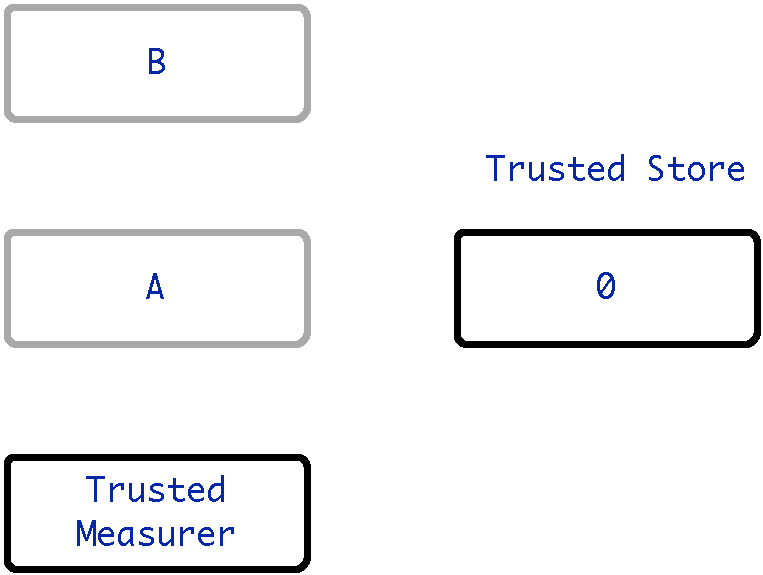
\includegraphics[width=1.0\textwidth]{figures/chain-root.pdf}}
      \only<2>{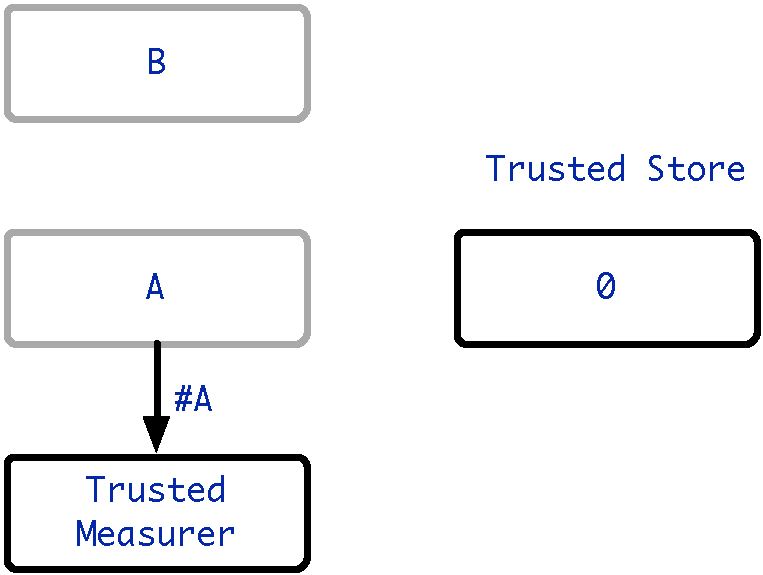
\includegraphics[width=1.0\textwidth]{figures/chain-measure.pdf}}
      \only<3>{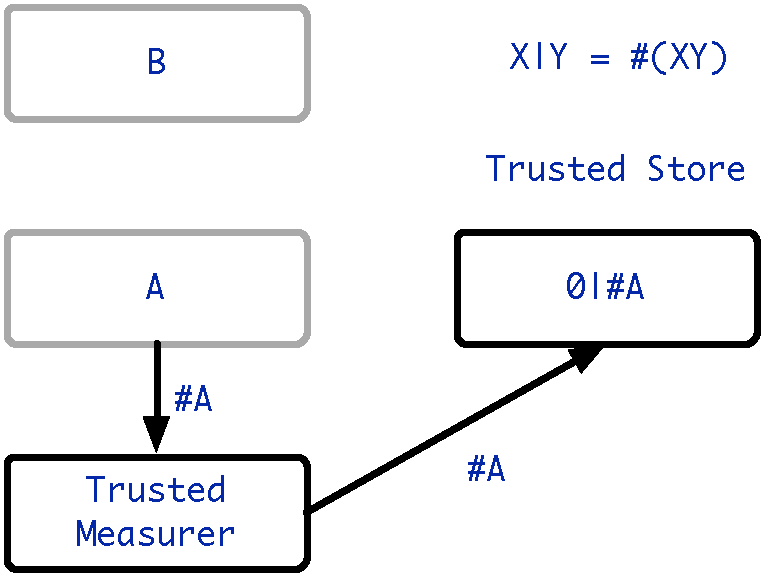
\includegraphics[width=1.0\textwidth]{figures/chain-store.pdf}}
      \only<4>{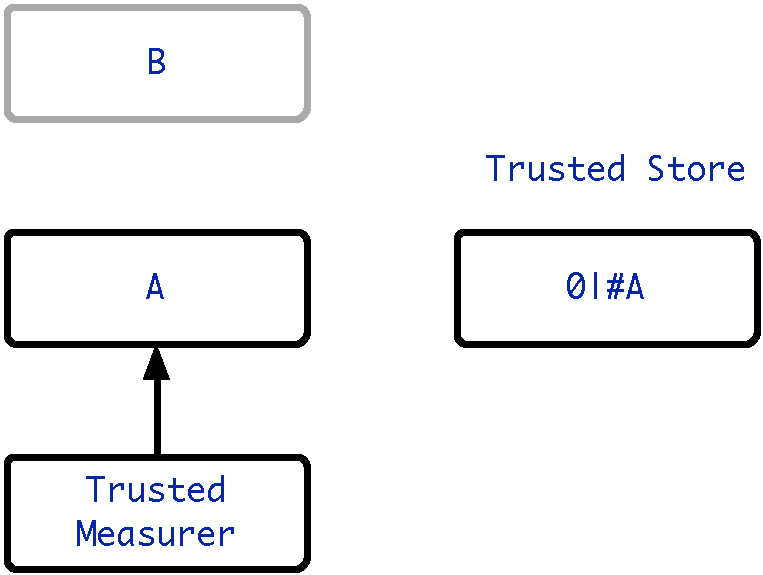
\includegraphics[width=1.0\textwidth]{figures/chain-start.pdf}}
      \only<5>{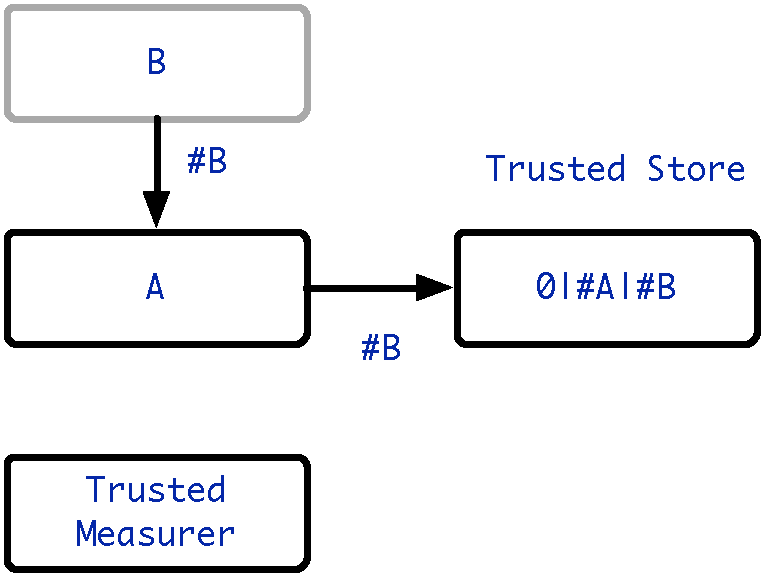
\includegraphics[width=1.0\textwidth]{figures/chain-next.pdf}}
      \only<6>{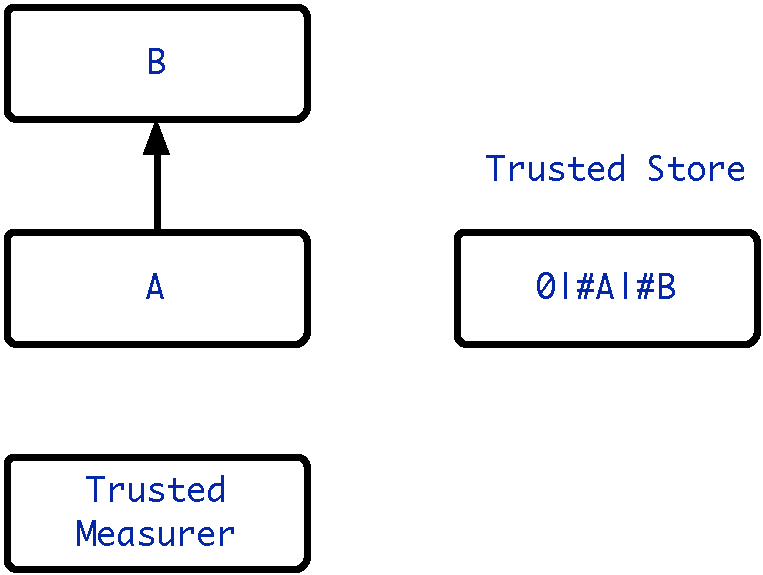
\includegraphics[width=1.0\textwidth]{figures/chain-final.pdf}}
    \end{figure}
  \end{columns}
}

\frame{\frametitle{Appraisal --- What Do We Know?}

  Measurement $\neq$ trust --- Measurements must be appraised

  \begin{itemize}
  \item Determine if $\extend{\extend{0}{\hash{A}}}{\hash{B}}$ is correct
    \begin{itemize}
    \item Calculate a \emph{golden hash} from $A$ and $B$
    \item Compare golden hash with
      $\extend{\extend{0}{\hash{A}}}{\hash{B}}$ from trusted store
    \item Correct $\extend{\extend{0}{\hash{A}}}{\hash{B}}$ implies
      trusted boot
    \end{itemize}
  \item Correct $\extend{\extend{0}{\hash{A}}}{\hash{B}}$ implies $A$ and $B$ must be correct
    \begin{itemize}
    \item Correct $\extend{\extend{0}{\hash{A}}}{\hash{B}}$ implies $\hash{A}$ and $\hash{B}$ are the correct hashes
    \item Correct $\hash{A}$ and $\hash{B}$ implies $A$ and $B$ are the correct binaries
    \item $A$ includes hash and launch functions
    \end{itemize}
  \item Correct $\extend{\extend{0}{\hash{A}}}{\hash{B}}$ implies measurement occurred in the right order
    \begin{itemize}
    \item $\hash{(XY)}\neq\hash{(YX)}$
    \item Trusted store started with 0
    \end{itemize}
  \end{itemize}
}

\frame{\frametitle{Appraisal --- But Why Trust B?}
  
  A chain exists from the Trusted Measurer and Trusted Store to B

  \begin{itemize}
  \item Trusted Measurer and Trusted Store are trusted \emph{a priori}
  \item A is trusted to be A because its measurement is:
    \begin{itemize}
    \item Correct
    \item Taken by a trusted party (Trusted Measurer)
    \item Stored by a trusted party (Trusted Store)
    \end{itemize}
  \item B is trusted to be B because its measurement is:
    \begin{itemize}
    \item Correct
    \item Taken by a trusted party (A)
    \item Stored by a trusted party (Trusted Store)
    \item If A's ability to measure B were compromised, $\hash{A}$
      would be wrong
    \end{itemize}
  \item and so on and so on...
  \end{itemize}
}

\frame{\frametitle{Trust is a Preorder}

  $\trusts{x}{y}$ is an homogeneous relation over actors that is true
  when \emph{x trusts y}.  $\trusts{x}{y}$ is by definition a preorer:

  \begin{itemize}
  \item Reflexive --- $\forall x \cdot \trusts{x}{x}$
  \item Transitive --- $\forall x,y,z\cdot\trusts{x}{y}\wedge\trusts{y}{z}  \Rightarrow
  \trusts{x}{z}$
  \end{itemize}

Measured Boot gathers evidence to check trust relationships.
}

\frame{\frametitle{Trust is a Preorder}

A \emph{chain of trust} from $X_0$ to $X_n$:

\[\trusts{X_0}{X_1}\wedge\trusts{X_1}{X_2}\wedge\ldots\wedge\trusts{X_{n-1}}{X_n}\]

\begin{itemize}
\item If $X_0$ is trusted, then $X_n$ is trusted
\item $X_0$ is called a \emph{root-of-trust}
\item Establishing trust chains defines a framework for measurement
\item Measurement provides evidence that trust chains are not violated
\item Appraisal checks evidence to assess trust chains
\end{itemize}

}

\frame{\frametitle{Trusted Platform Module}
  The \emph{Trusted Platform Module (TPM)} is a cryptographic
  coprocessor for trust.

  \begin{itemize}
  \item Endorsement Key (EK) --- factory generated asymmetric key
    that uniquely identifies the TPM
  \item Attestation Instance Key (AIK) ---
    \texttt{TPM\_CreateIdentity} generated asymmetric key alias for
    the EK
  \item Storage Root Key (SRK) --- \texttt{TPM\_TakeOwnership}
    generated asymmetric key that encrypts data associated with the
    TPM
  \item Platform Configuration Registers (PCRs) --- protected
    registers for storing and extending hashes
  \item NVRAM --- Non-volatile storage associated with the TPM
  \end{itemize}
}

\frame{\frametitle{Endorsement Key}
  \begin{itemize}
  \item Asymmetric key generated at TPM fabrication
  \item $\private{EK}$ is protected by the TPM
  \item $\public{EK}$ by convention is managed by a Certificate
    Authority
    \begin{itemize}
    \item Binds $\public{EK}$ with a platform
    \item Classic trusted third party
    \end{itemize}
  \item Only used for encryption
  \item Attestation Instance Keys (AIK) are aliases for the EK
    \begin{itemize}
    \item Used for signing
    \item Authorized by the EK
    \end{itemize}
  \end{itemize}
}

\frame{\frametitle{Storage Root Key}
  \begin{itemize}
  \item Asymmetric key generated by \texttt{TPM\_TakeOwnership}
  \item $\private{SRK}$ is protected by the TPM
  \item $\public{SRK}$ is available for encryption
  \item Used as the root for chaining keys by \emph{wrapping}
    \begin{itemize}
    \item A wrapped key is an asymmetric key pair with it's private
      key sealed
    \item Safe to share the entire key
    \item Only usable in the presence of the wrapping key with
      expected PCRs
    \end{itemize}
  \end{itemize}
}

\frame{\frametitle{Platform Configuration Registers}
  \begin{itemize}
  \item Operations on PCRs
    \begin{itemize}
    \item Extension --- Hash a new value juxtaposed with the existing
      PCR value
    \item Reset --- Set to 0
    \item Set --- Set to a known value
    \end{itemize}
  \item Operations using PCRs
    \begin{itemize}
    \item Sealing data --- PCR state dependent encryption
    \item Wrapping keys --- PCR state dependent encryption of a
      private key
    \item Quote --- Reporting PCR values to a third party
    \end{itemize}
  \item Properties
    \begin{itemize}
    \item Locality --- Access control like OS security rings
    \item Resettable --- PCR can be reset to known value after \emph{SENTER}
    \item Many others that we don't need yet
    \end{itemize}
  \end{itemize}
}

\frame{\frametitle{Resetting PCRs}
  \begin{block}{Non-Resettable}
    \begin{itemize}
    \item History since reboot
    \item Reset only on reboot
    \item Good for recording trajectory
    \end{itemize}
  \end{block}
  \begin{block}{Resettable}
    \begin{itemize}
    \item No history
    \item Reset before use
    \item Good for one-off user data
    \end{itemize}
  \end{block}

  \begin{itemize}
  \item Reset requires appropriate permissions based on locality
  \item A PCR is resettable if defined in platform spec
  \end{itemize}
}

\frame{\frametitle{Locality}

  \begin{block}{Locality = Access Control for PCRs}
    \begin{itemize}
    \item Each PCR is assigned a locality
    \item Only processes with locality greater than or equal a PCR's
      locality may modify it
    \item Increases monotonically starting at \texttt{SENTER} invocation
    \end{itemize}
  \end{block}


  \begin{block}{Locality and What Runs There}
  \begin{tabular}{ll}
    \emph{Locality} & \emph{Purpose} \\ \hline\hline
    4 & Trusted Hardware/SINIT Policy \\
    3 & Other MLE Components \\
    2 & Operating System \\
    1 & Applications Static \\
    0 & RTM/Legacy \\
  \end{tabular}
  \end{block}
}

\frame{\frametitle{Locality Rules of Thumb}

  \begin{itemize}
  \item Only SENTER runs in locality 4
  \item Only SINIT runs in locality 3
  \item OS and core system run in locality 2
  \item Applications run in locality 1
  \item Locality 0 is rarely used
  \end{itemize}
}

\frame{\frametitle{Roots of Trust} 

  A \emph{root of trust} provides a basis for transitively building
  trust.  Roots of trust are trusted implicitly. 
  \\
  There are three important Roots of Trust:
  
  \begin{itemize}
  \item Root of Trust for Measurement (RTM)
  \item Root of Trust for Reporting (RTR)
  \item Root of Trust for Storage (RTS)
  \end{itemize}
}

\frame{\frametitle{Root of Trust for Measurement}
  A \emph{Root of Trust for Measurement} is trusted to take the base
  system measurement.

  \begin{itemize}
  \item A hash function called on an initial code base from
    a protected execution environment
  \item Starts the measurement process during boot
  \item In the Intel TXT process the RTM is \texttt{SENTER}
    implemented on the processor
  \end{itemize}
}

\frame{\frametitle{Root of Trust for Reporting}
  A \emph{Root of Trust for Reporting} is trusted to guarantee the
  integrity of the base system report or quote

  \begin{itemize}
  \item A protected key used for authenticating reports
  \item In the Intel TXT processes this is the TPM's Endorsement Key
    (EK)
  \item Created and bound to its platform by the TPM foundry
  \item $\private{EK}$ is stored in the TPM and cannot be accessed by
    any entity other than the TPM
  \item $\public{EK}$ is available for encrypting data for the TPM
  \item $\private{EK}$ is used for decrypting data inside the TPM
  \item Linking $\public{EK}$ to its platform is done by a trusted
    Certificate Authority (CA)
  \end{itemize}
}

\frame{\frametitle{Root of Trust for Storage}
  A \emph{Root of Trust for Storage} is trusted to protect stored data

  \begin{itemize}
  \item A key stored in a protected location
  \item In the Intel TXT boot process this is the TPM's Storage Root
    Key (SRK)
  \item Created by \texttt{TPM\_TakeOwnership}
  \item $\private{SRK}$ is stored in the TPM and cannot be accessed by
    any entity other than the TPM
  \item $\public{SRK}$ is available for encrypting data for the TPM
  \item SRK is used for protecting other keys
  \end{itemize}
}

\frame{\frametitle{One Step from Roots of Trust}
  
  Roots of trust are used to build a trusted system from boot.

  \begin{columns}[c]
    \column{.53\textwidth}
    \begin{itemize}
    \item<1-> Power-on reset
    \item<2-> Resettable PCRs set to -1
    \item<3-> \texttt{SENTER} called, resets resettable PCRs to 0
    \item<4-> \texttt{SENTER} measures \texttt{SINIT} policy into PCR 18
    \end{itemize}
    \column{.45\textwidth}
    \begin{figure}
      \only<1>{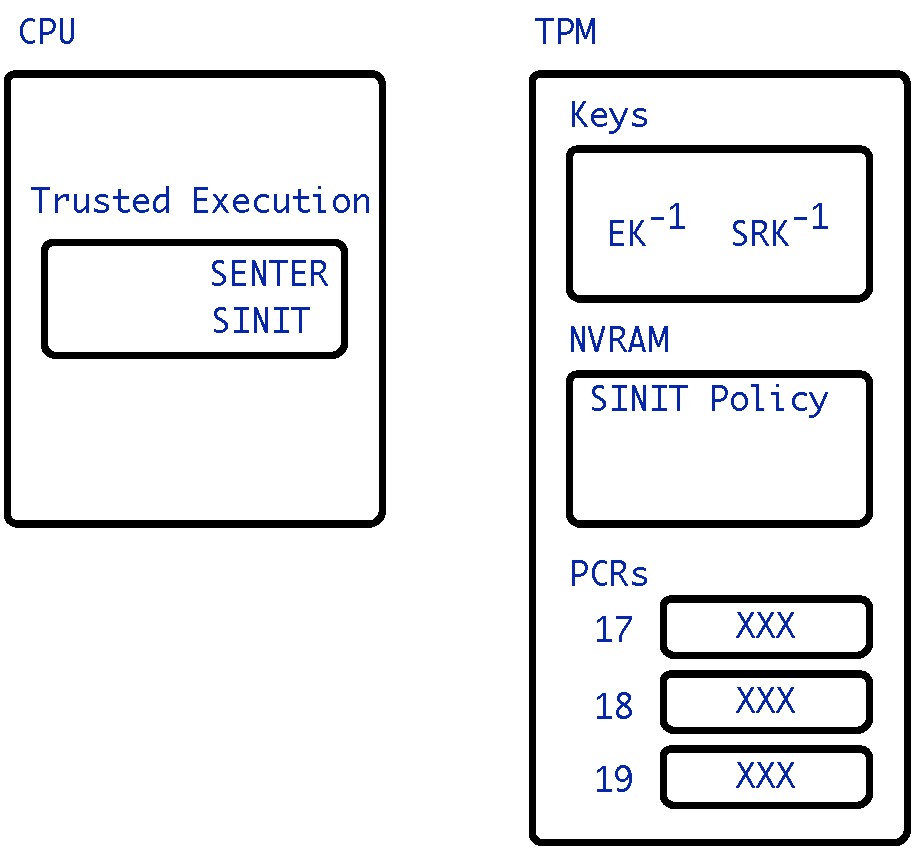
\includegraphics[width=1.0\textwidth]{figures/boot-pre-reset.pdf}}
      \only<2>{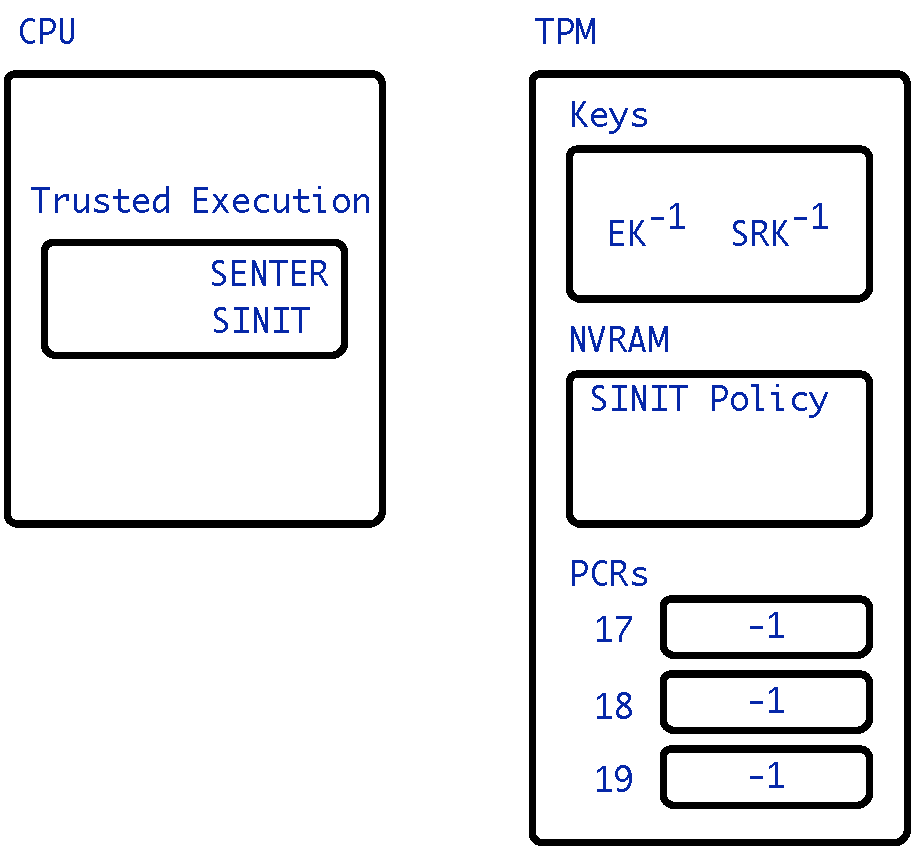
\includegraphics[width=1.0\textwidth]{figures/boot-reset.pdf}}
      \only<3>{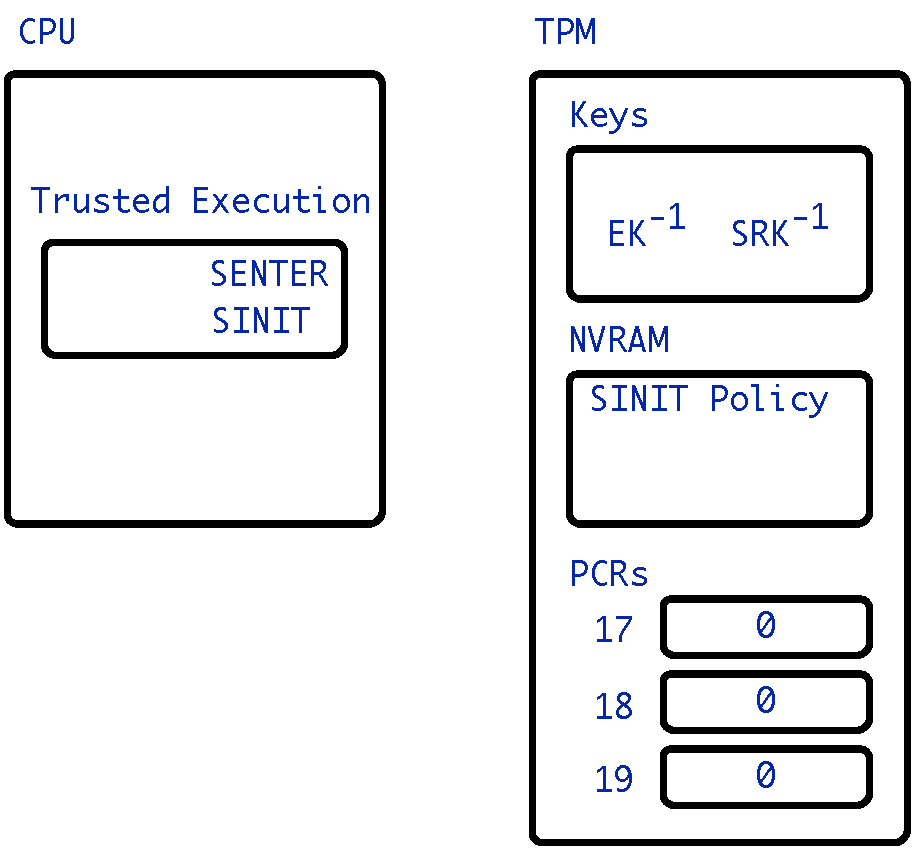
\includegraphics[width=1.0\textwidth]{figures/boot-senter.pdf}}
      \only<4>{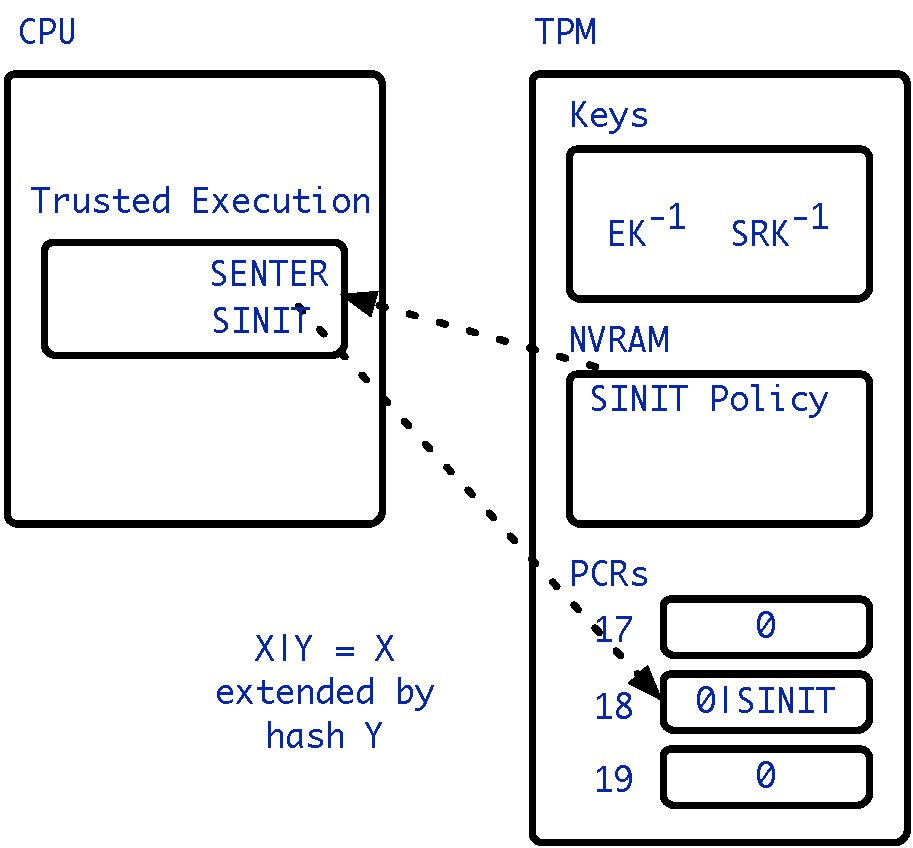
\includegraphics[width=1.0\textwidth]{figures/boot-senter-post.pdf}}
    \end{figure}
  \end{columns}
}

\frame{\frametitle{What We Know From Good PCR 18}
  A good value in PCR 18 tells us:

  \begin{itemize}
  \item \texttt{SENTER} was called --- Resetting PCR 18 starts
    measurements at 0 rather than -1
  \item \texttt{SINIT} was measured by \texttt{SENTER} --- Only
    \texttt{SENTER} can extend PCR 18
  \item \texttt{SINIT} uses the correct policy --- PCR 18 is extended
    with \texttt{SINIT} measurement policy
  \item \texttt{SENTER} ran before \texttt{SINIT} was measured ---
    $\extend{A}{B} \neq \extend{B}{A}$
  \end{itemize}

  \begin{block}{Measurement $\neq$ Trust}
    Measurements must be appraised to determine trust.
  \end{block}
}

\frame{\frametitle{Two Steps from Roots of Trust}

  \begin{columns}[c]
    \column{.53\textwidth}
    \begin{itemize}
    \item<1-> \texttt{SINIT} measures the Measured Launch Environment (MLE)
      using measured \texttt{SINIT} policy
    \item<1-> \texttt{SINIT} returns control to \texttt{SENTER}
    \item<2-> \texttt{SENTER} invokes the MLE
    \end{itemize}
    \column{.45\textwidth}
    \begin{figure}
      \only<1>{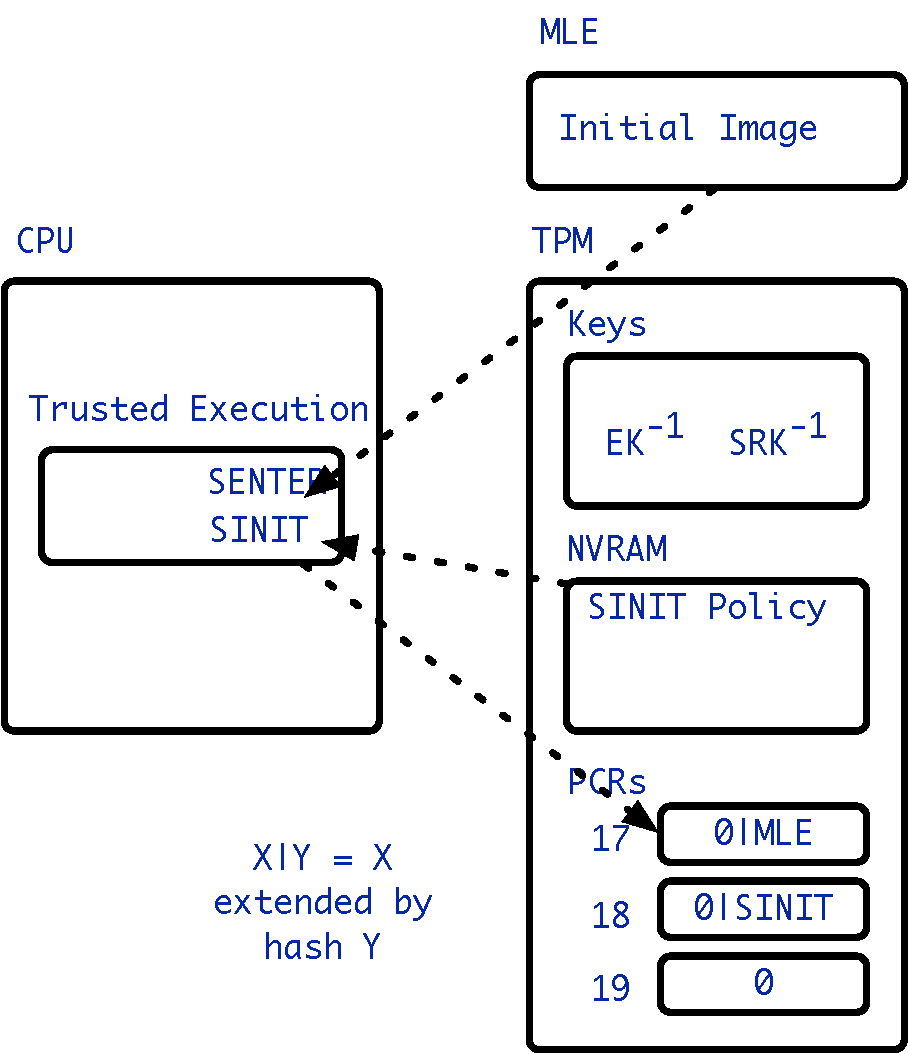
\includegraphics[width=1.0\textwidth]{figures/boot-pre-sinit.pdf}}
      \only<2>{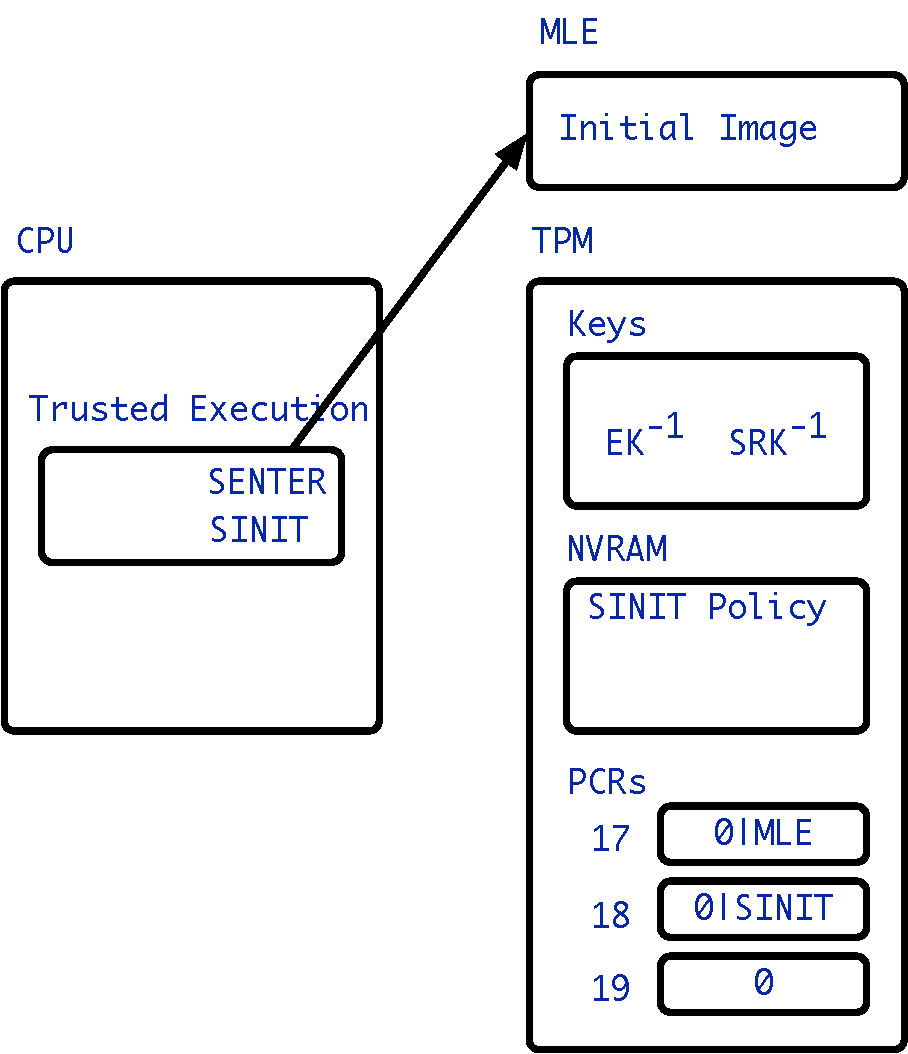
\includegraphics[width=1.0\textwidth]{figures/boot-sinit-post.pdf}}
    \end{figure}
  \end{columns}
}

\frame{\frametitle{What We Know From Good PCRs}
  \begin{itemize}
  \item \texttt{SENTER} was called --- Resetting PCR 18 starts
    measurement sequence at 0 rather than -1
  \item \texttt{SINIT} policy was measured by \texttt{SENTER} --- Only
    \texttt{SENTER} can extend PCR 18
  \item \texttt{SINIT} uses the correct policy --- PCR 18 is extended
    with \texttt{SINIT} measurement policy
  \item \texttt{SENTER} ran before \texttt{SINIT} ---
    $\extend{0}{\hash{SINIT}}\neq\extend{-1}{\hash{SINIT}}$
  \item \texttt{MLE} is good --- Measured by good \texttt{SINIT} into
    PCR
  \end{itemize}

  \begin{block}{Boot is generic until the \texttt{MLE} starts}
    MLE is the beginnings of the operating system.
  \end{block}
}

\frame{\frametitle{Boot the MLE}
  \begin{columns}[c]
    \column{.53\textwidth}
    \begin{itemize}
      \item<1-> \texttt{SENTER} starts the MLE 
        \begin{itemize}
        \item<1-> \texttt{SENTER} starts the initial image
        \item<1-> Initial image starts the system
        \end{itemize}
      \item<2-> Initial image initialized the kernel
        \begin{itemize}
        \item<2-> Measures the kernel into the TPM
        \item<2-> Starts the kernel
        \end{itemize}
      \item<3-> Kernel boots the system
        \begin{itemize}
        \item<3-> Measures remaining images into the TPM
        \item<3-> Starts remaining images
        \item<3-> Measures application into the TPM
        \item<3-> Starts the application
        \end{itemize}
    \end{itemize}
    \column{.45\textwidth}
    \begin{figure}
      \only<1>{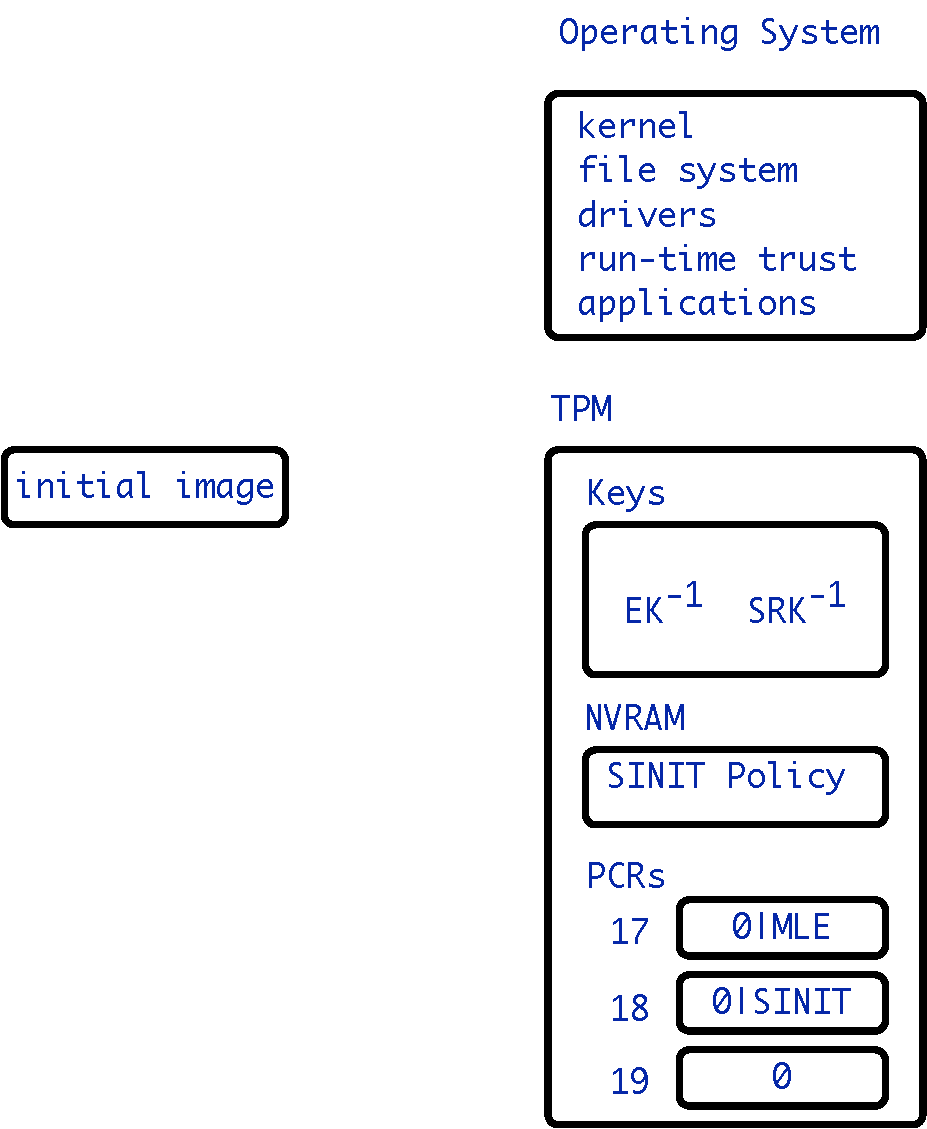
\includegraphics[width=1.0\textwidth]{figures/boot-pre-hypervisor.pdf}}
      \only<2>{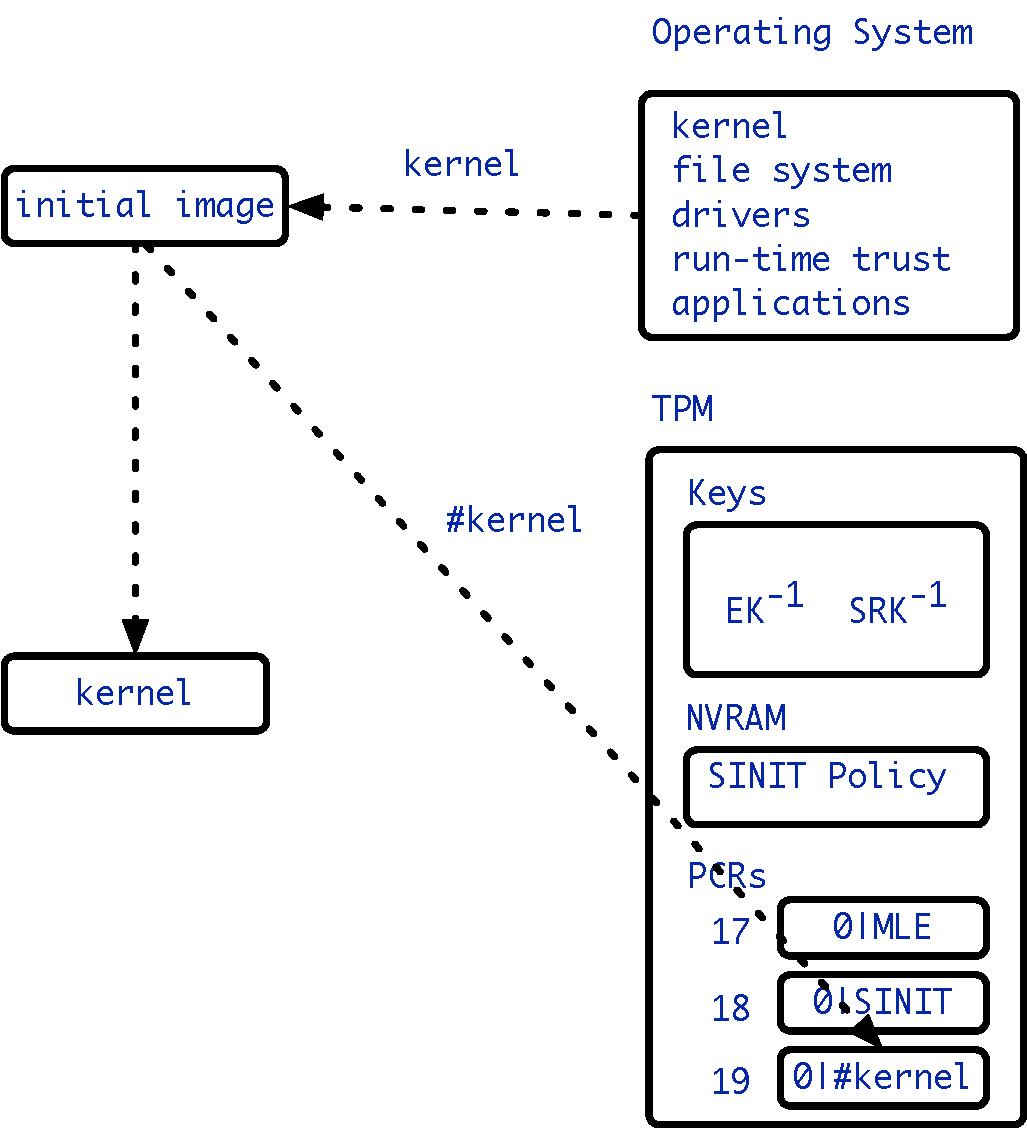
\includegraphics[width=1.0\textwidth]{figures/boot-vtpm.pdf}}
      \only<3>{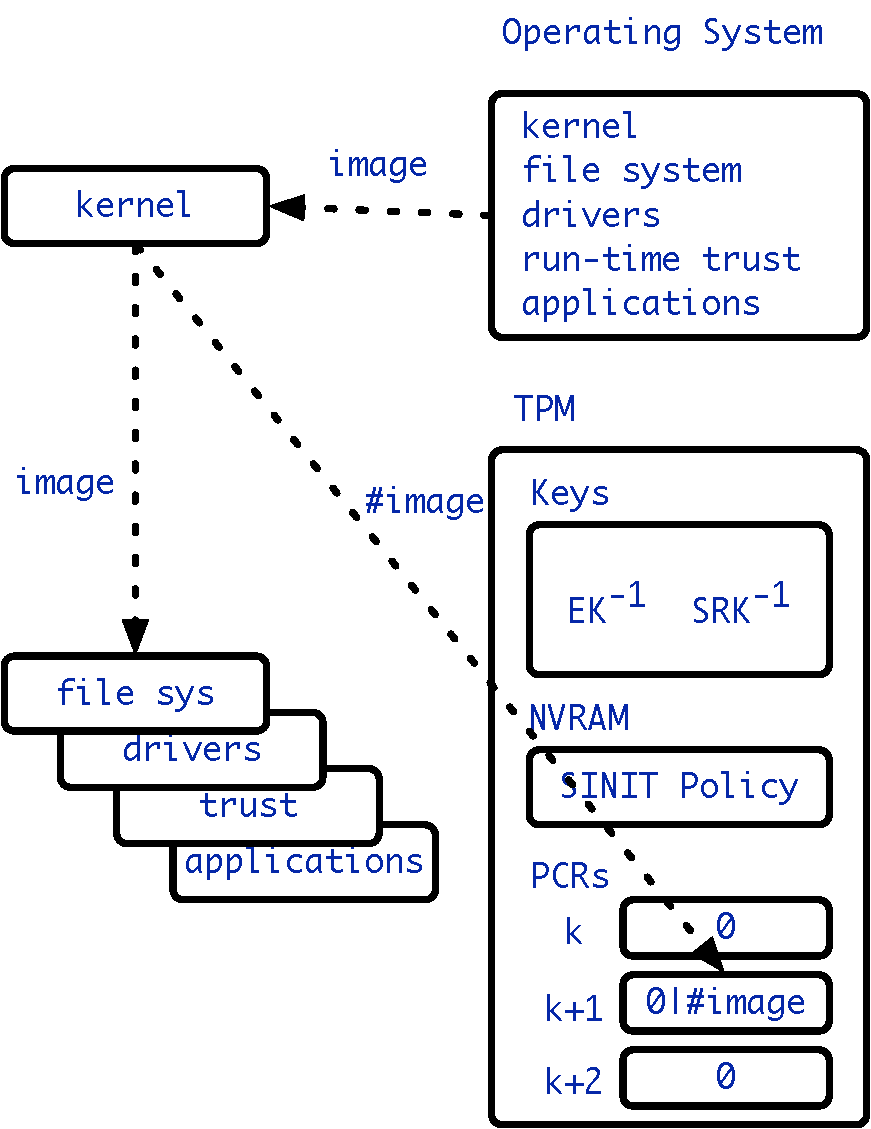
\includegraphics[width=1.0\textwidth]{figures/boot-platform.pdf}}
      \only<4>{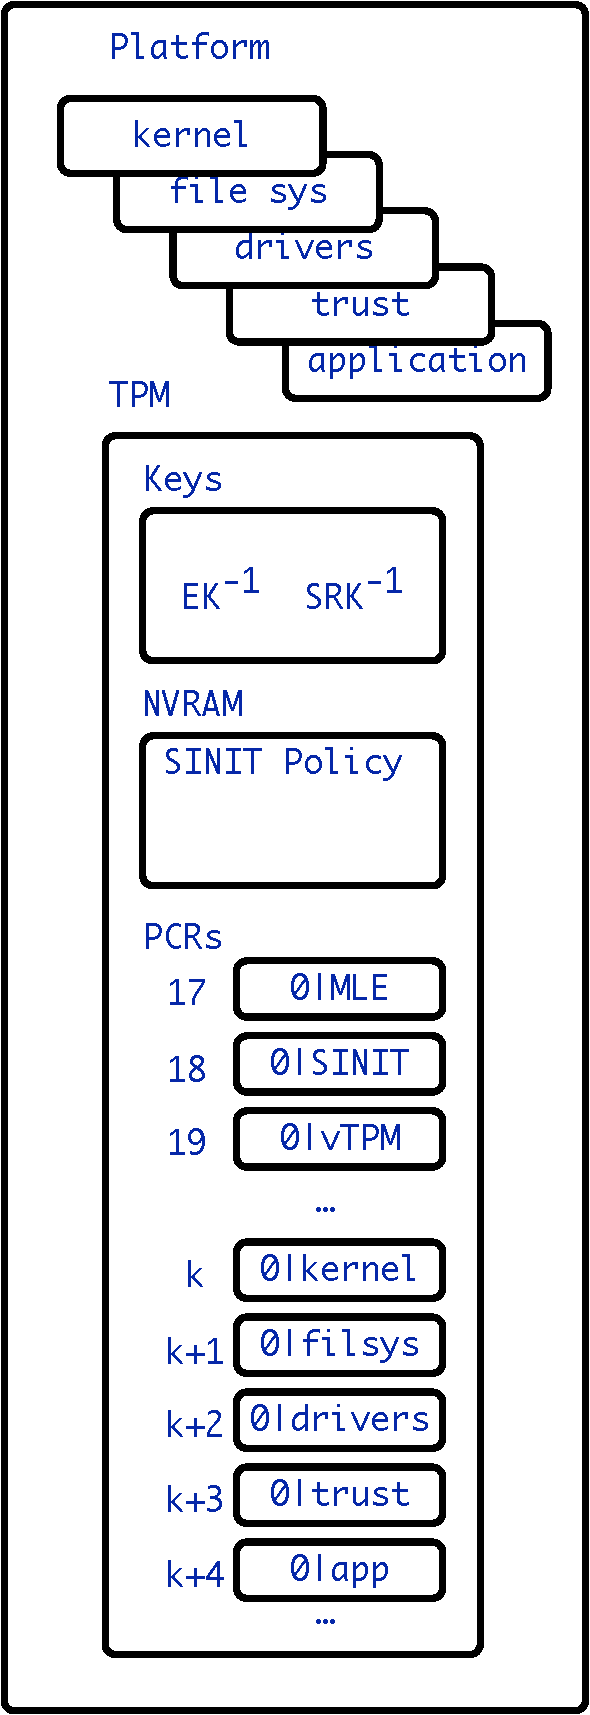
\includegraphics[width=0.5\textwidth]{figures/boot-platform-post.pdf}}
    \end{figure}
  \end{columns}
}


\frame{\frametitle{What we know from good PCRs}
  

  \begin{block}{Built from Good Parts}
    We can construct a proof that the platform is constructed correctly
    from PCR contents
  \end{block}

  \begin{itemize}
  \item SINIT measured the right initial image - PCR 18 measurement
    and we trust \texttt{SENTER}
  \item The right initial image started - PCR 17 measurement and
    we trust \texttt{SENTER}, \texttt{SINIT} and \texttt{SINIT} Policy
    is measured
  \item The right kernel started - PCR 19 measurement and we trust
    \texttt{SENTER}, \texttt{SINIT}, and initial image is measured
  \item The right system components started - PCRs and
    the kernel is measured
  \item The right application started - TPM PCRs and the kernel is measured
  \end{itemize}
}

\frame{\frametitle{Chaining Trust (Reprise)}
  \begin{itemize}
  \item Trust is transitive
    \begin{itemize}
    \item $\trusts{x}{y} \wedge \trusts{y}{z} \Rightarrow
      \trusts{x}{z}$
    \item Construct evidence trust chains
    \item Remember ``directly observed or indirectly observed by a
      trusted third party''
    \end{itemize}
  \item Roots of Trust define the ``root'' for trust
    \begin{itemize}
    \item Use Roots of Trust to establish base for chain
    \item SENTER/SINIT is the Trusted Measurer
    \item SRK and TPM is the Trusted Storage Root (Unused so far)
    \item EK and TPM is the Trusted Reporter (Coming next)
    \end{itemize}
  \item Extend chains of trust by measuring before executing
  \end{itemize}
}

\frame{\frametitle{Getting a Quote}
  
  A \emph{quote} is a signed data package generated by a TPM used to
  establish trust 

  \begin{itemize}
  \item $q=\sign{\langle n,pcr\rangle}{AIK}$
    \begin{itemize}
    \item $n$ - A nonce or other data
    \item $pcr$ - A PCR composite generated from TPM PCRs
    \item $\private{AIK}$ - An alias for $\private{EK}$ used for
      signing instead of $\private{EK}$
    \end{itemize}
    \item Generated by the TPM with command \texttt{TPM\_Quote}
  \end{itemize}
}

\frame{\frametitle{Attestation Identity Key}

  An $\public{AIK}$ is A wrapped TPM key bound to an $\private{EK}$
  usable only in the TPM that generated it in the right state

  \begin{itemize}
  \item $\encrypt{\seal{\private{AIK}}{pcr}}{\private{EK}}$ - the
    $\private{AIK}$ encrypted with $\private{EK}$ and sealed to
    $pcr$ values.
  \item $\encrypt{\seal{\private{AIK}}{pcr}}{\private{EK}}$ decrypts
    and installs only when
    \begin{itemize}
    \item $pcr$ matches the TPM's PCRs at decryption time
    \item $\private{EK}$ is the TPM's endorsement key
    \end{itemize}
  \item Protected by a combination of encryption and state
  \item Generated by a TPM
  \end{itemize}
}

\frame{\frametitle{Appraising a Quote}
  
  Given $q$ of the form:

  \[q=\sign{\langle n,pcr\rangle}{AIK}\]
  
  \begin{enumerate}
  \item Signature check using $\public{AIK}$ verifies authenticity
    \begin{itemize}
    \item Signature was generated by a TPM with AIK installed
    \item Appraiser must know $\public{AIK}$
    \end{itemize}
  \item $pcr$ check verifies built from good parts in the right order
    \begin{itemize}
    \item Compare PCR composite to known good PCR composite
    \item Composite generated from desired golden PCR values
    \end{itemize}
  \item Nonce check guarantees freshness
    \begin{itemize}
    \item Nonce is random and known to the appraiser
    \item Sent to the target during appraisal
    \end{itemize}
  \end{enumerate}
}

\frame{\frametitle{Certifying AIK}
  
  Assume a trusted Certificate Authority (CA) that maintains links from ID
  to $\public{EK}$ with well-known public key $\public{CA}$

  \begin{columns}[c]
    \column{.53\textwidth}
    \begin{itemize}
    \item<1-> $ID_n$ requests $\public{AIK}$ certification from CA
    \item<2-> CA signs $\public{AIK}$ with $\private{CA}$
    \item<3-> CA encrypts $\sign{\public{AIK}}{CA}$ with $ID_n$'s $\public{EK_n}$
    \item<4-> CA sends $\encrypt{\sign{\public{AIK}}{CA}}{EK_n}$ to $ID_n$
    \item<5-> $ID_n$ decrypts encrypted AIK with $\private{EK_n}$
    \item<6-> $ID_n$ sends $\sign{\public{AIK}}{CA}$ to appraiser
    \end{itemize}
    \column{.45\textwidth}
    \begin{figure}
      \only<1>{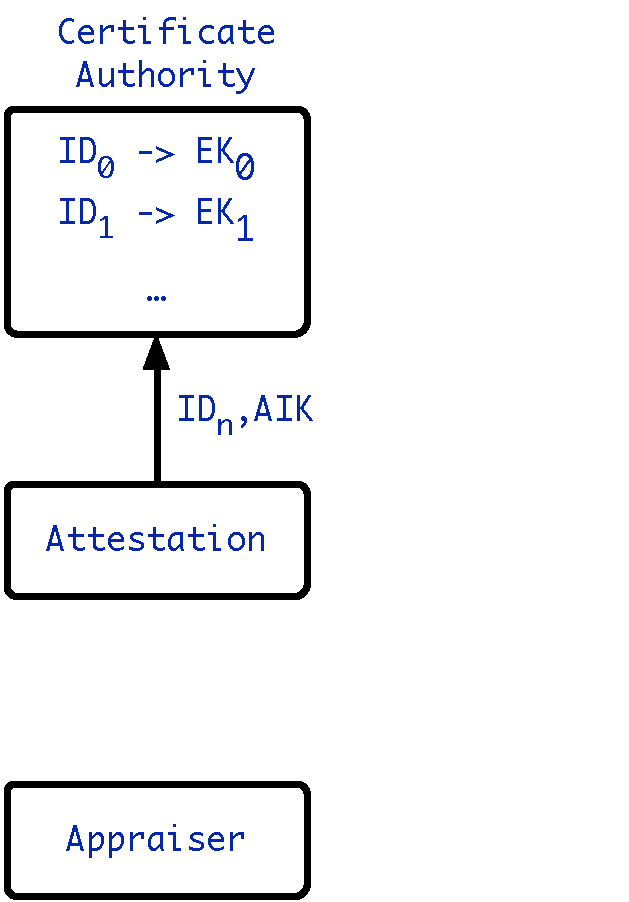
\includegraphics[width=0.70\columnwidth]{figures/cert-pre.pdf}}
      \only<2>{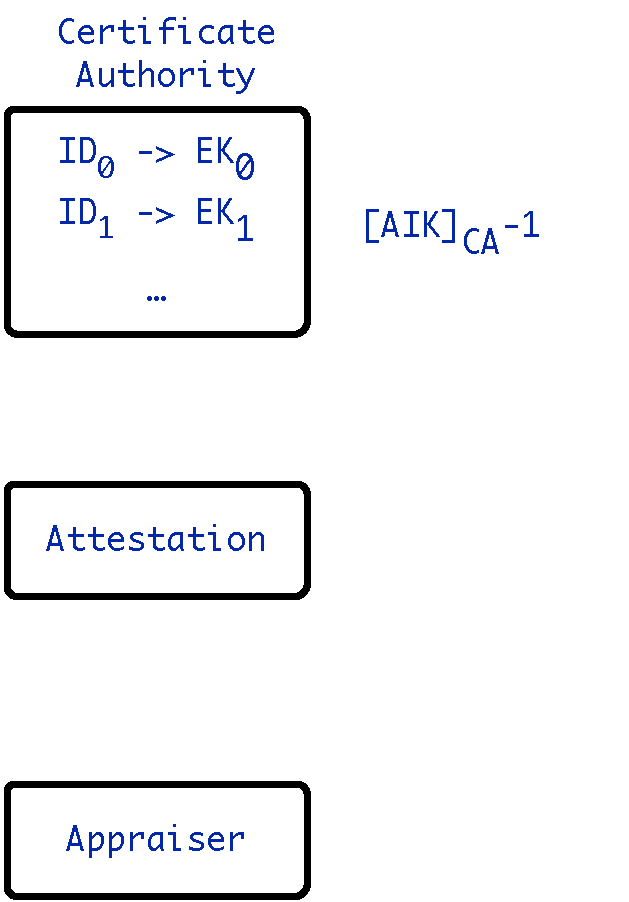
\includegraphics[width=0.70\columnwidth]{figures/cert-gen.pdf}}
      \only<3-4>{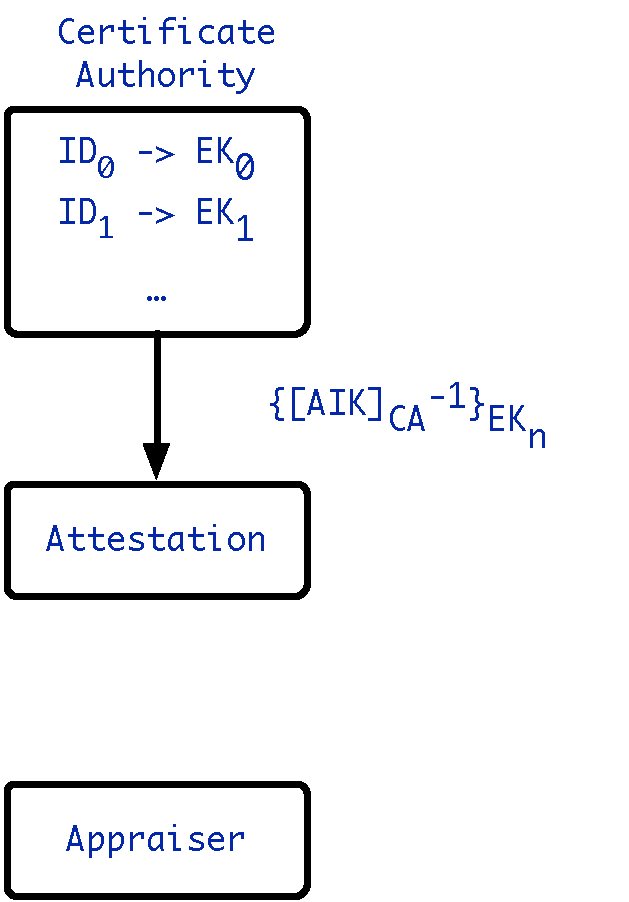
\includegraphics[width=0.70\columnwidth]{figures/cert-crypt.pdf}}
      \only<5-6>{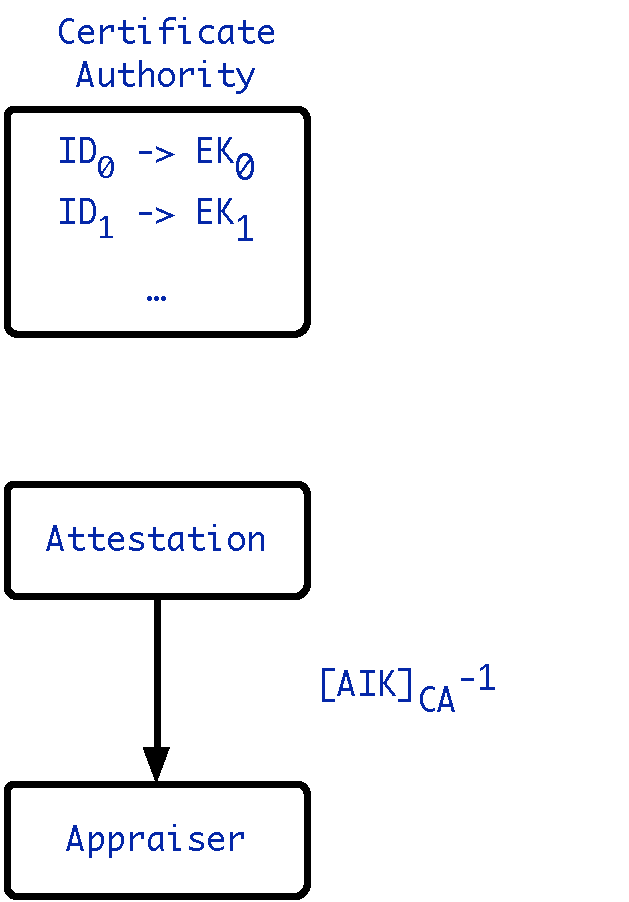
\includegraphics[width=0.70\columnwidth]{figures/cert-decrypt.pdf}}
    \end{figure}
  \end{columns}
}

\frame{\frametitle{Why Believe AIK Belongs to $ID_n$?}

  Cryptographic evidence ensures $\public{AIK}$ is an alias for the
  right $\public{EK}$

  \begin{itemize}
  \item Only the CA can generate $\sign{\public{AIK}}{CA}$
  \item CA is trusted to know $ID_n\rightarrow EK_n$
  \item CA is trusted to generate
    $\encrypt{\sign{\public{AIK}}{CA}}{EK_n}$
  \item Only $ID_n$ can decrypt $\encrypt{\sign{\public{AIK}}{CA}}{EK_n}$
  \item Appraiser can check $\sign{\public{AIK}}{CA}$ to ensure use of
    trusted CA
  \item If Appraiser can use $\public{AIK}$ then it was decrypted by
    $ID_n$
  \end{itemize}

  \alert{AIK is now a certified alias for EK used for signing}
}

\frame{\frametitle{Using Protocol Notation}

  Protocol notation specifies communication:

  \[\msg{Sender}{Receiver}{Messsage}\]

  \begin{block}{Key Certification Protocol}
  \begin{eqnarray}
    \begin{aligned}
    & \msg{ID_n}{CA}{AIK} \\
    & \msg{CA}{ID_n}{\encrypt{\sign{\public{AIK}}{CA}}{EK_n}} \\
    & \msg{ID_n}{App}{\sign{\public{AIK}}{CA},\sign{\langle n,pcr\rangle}{\public{AIK}}}
    \end{aligned}
  \end{eqnarray}
  \end{block}
}

\frame{\frametitle{Remote Data Acquisition}

  Boot and appraise remote system for covert data acquisition

  \begin{itemize}
    \item Target reset triggers target boot initialization
    \item Target initial boot goes through BIOS and device startup
    \item Target secondary boot establishes comm link and ``phones home''
    \item Appraiser evaluates target
    \item Appraiser responds to target with OS image
    \item Target boots OS image
    \item Target begins operation
    \item Appraiser evaluates target
    \item Target begins data acquisition and transmission
  \end{itemize}
}

\frame{\frametitle{Assumptions}

  General assumptions:

  \begin{itemize}
  \item Nonces, keys and hashes cannot be guessed
  \item Perfect cryptography
  \item All messages are carried by the adversary
  \end{itemize}

  System specific assumptions:

  \begin{itemize}
  \item Secure communication subsystem is trustworthy
  \item Target knows what to communicate with
  \item TPM present on the target
  \item AIK is established and certified prior to system launch
  \end{itemize}

}

\frame{\frametitle{Designing A Trusted System}

  What assets should be protected and how?

  \begin{itemize}
  \item What assets must be handled confidentially?
  \item What assets must be handled with integrity?
  \item What assets and behaviors must be appraised?
  \item What behaviors must be prevented?
  \end{itemize}

  Some initial observations:

  \begin{itemize}
  \item Initial boot software - integrity, must be appraised
  \item Communication addresses - confidentiality
  \item Hardware and tamper protections - integrity, must be appraised
  \item Operating system - integrity, must be appraised
  \item Data transmission key - confidentiality
  \end{itemize}

}

\frame{\frametitle{Trust}

\begin{block}{Trust is:}
  \begin{itemize}
  \item Strong identification
  \item Direct observation of good behavior
  \item Indirect observation of good behavior by a trusted third party
  \end{itemize}
\end{block}

\begin{block}{Late Launch is:}
  \begin{itemize}
  \item Initial measurement taken and stored by roots of trust for
    measurement and storage
  \item Reporting performed by root of trust for reporting
  \item Trust chains transitively from roots of trust outward
  \item System is constructed of good parts
  \end{itemize}
\end{block}

}

\frame{\frametitle{Roots of Trust}
  \begin{itemize}
  \item Root of trust for measurement
    \begin{itemize}
    \item SENTER for launch
    \item Initial measurement taken by SINIT
    \item Hardware-based TPM initialization
    \end{itemize}
  \item Root of trust for storage
    \begin{itemize}
    \item TPM storage root key (SRK)
    \item Locality enforcement
    \item TPM separation
    \end{itemize}
  \item Root of trust for reporting
    \begin{itemize}
    \item TPM endorsement key (EK)
    \item TPM separation
    \end{itemize}
  \end{itemize}
}

\frame{\frametitle{Initial Design Decisions}

  \begin{block}{Design Decisions}
    \begin{itemize}
    \item What are measurement responsibilities?
    \item What is in the MLE?
    \item Where are measurements stored?
    \item How is locality assigned?
    \end{itemize}
  \end{block}

}

\frame{\frametitle{Measurement Responsibilities}
  
  \begin{itemize}
  \item \texttt{SENTER} measures \texttt{SINIT} policy
  \item \texttt{SINIT} measures the Measured Launch Environment (MLE)
  \item Initial boot measures hardware and Secondary boot software
  \item Secondary boot measures OS
  \item OS measures components as they start
  \end{itemize}
  
  \begin{block}{Measurement Relation}
    \[
    \mathtt{SENTER} \rightarrow \mathtt{SINIT} \rightarrow
    \mathtt{MLE} \rightarrow \mathtt{OS} \rightarrow \mathtt{app}
    \]
  \end{block}

  \begin{itemize}
  \item No measurement loops
  \item Everything is measured
  \end{itemize}

}


\frame{\frametitle{Traditional Measurement Storage}

  \begin{tabular}{ll}
    \emph{PCR} & \emph{Contents} \\ \hline
    0--15 & Static RTM \\
    16 & Debug \\
    17 & Locality 4 measurements by \texttt{SENTER} \\
    18 & Locality 3 measurements by \texttt{SINIT} \\
    19 & Locality 2 measurements by MLE and OS \\
    20 & Locality 1 measurements by applications \\
    21--22 & T/OS controlled \\
    23 & Application specific measurements \\
  \end{tabular}

\begin{block}{Need a PCR?}
\begin{itemize}
\item Available non-resettable PCRs are 8-15
\item Available resettable PCRs are 16,23
\end{itemize}
\end{block}

}

\frame{\frametitle{What is in the MLE?}

  \begin{itemize}
  \item Anything measured by SINIT is in the MLE by definition
  \item MLE could be the initial boot image or the entire boot image
  \item How much granularity desired in measurements?
  \end{itemize}

  \begin{block}{What is in the MLE?}
    \begin{itemize}
    \item Initial boot image
    \item Nothing more
    \end{itemize}
  \end{block}

}

\frame{\frametitle{Where Are Measurements Stored?}

  \begin{itemize}
  \item Initial measurement storage location is standard
  \item Typically 1 hash per measurement, but could be a sequence
  \end{itemize}

  \begin{block}{PCRs 17 and 18}
  \begin{itemize}
  \item SINIT Policy measured by \texttt{SENTER} into PCR 17
  \item MLE Measured by \texttt{SINIT} into PCR 18
  \item PCRs 17 \& 18 are non-resettable
  \end{itemize}
  \end{block}
}

\frame{\frametitle{Where Are Measurements Stored?}
  \begin{itemize}
  \item Later measurements must be designed
  \item One big hash, many hashes, one PCR, many PCRs
  \end{itemize}

  \begin{block}{PCRs 19 and 20}
    \begin{itemize}
    \item OS measured into PCR 19
    \item Application(s) measured into PCR 20
    \end{itemize}
  \end{block}
}

\frame{\frametitle{What are the Measurements?}
  \begin{itemize}
  \item Measure the OS
    \begin{itemize}
    \item OS measured as one hash
    \item OS measured as a hash sequence by the OS startup
    \end{itemize}
  \item Applications measured as one hash each
  \item Ordering application measurement?
    \begin{itemize}
    \item Enforce application hash order by sequencing startup
    \item Use multiple PCRs
    \item Produce multiple good hashes in appraiser
    \end{itemize}
  \item Measurement \emph{must} be performed as components are started
  \end{itemize}
}

\frame{\frametitle{Measurement Options and Appraisal}
  
  \begin{itemize}
  \item Measurement granularity
    \begin{itemize}
    \item One hash says good or bad for all system binaries and is
      simple to take
    \item Many hashes extending a PCR says good or bad for all system
      binaries including order
    \end{itemize}
  \item One or Many PCRs
    \begin{itemize}
    \item One PCR says good or bad for all system binaries with order
    \item Many PCRs says good or bad for individual system binaries
      without order
    \end{itemize}
  \item Resettable or Non-Resettable
    \begin{itemize}
    \item Resettable ignores history prior to reset
    \item Non-resettable captures history from system startup
    \end{itemize}
  \end{itemize}

}

\frame{\frametitle{Where are Measurements Stored? (Redux)}

  \begin{itemize}
  \item Poky Linux is measured as one hash into PCR 19
    \begin{itemize}
    \item Need to know good or bad on startup
    \item Using Poky Linux unmodified
    \end{itemize}
  \item Application is measured as one hash into PCR 20
    \begin{itemize}
    \item Need to know good or bad on startup
    \item Only one application
    \end{itemize}
  \end{itemize}

  \begin{block}{PCRs 19 and 20}
    \begin{itemize}
    \item OS measured into PCR 19 by secondary boot prior to start
    \item Application(s) measured into PCR 20 by OS prior to start
    \end{itemize}
  \end{block}
}

\frame{\frametitle{How is Locality Assigned?}

  \begin{itemize}
  \item No reason to deviate from standard locality mapping
  \item No reason to reset PCRs
  \end{itemize}

  \begin{block}{Locality Assignment}
    \begin{itemize}
    \item PCR 17 - Locality 4, non-resettable
    \item PCR 18 - Locality 3, non-resettable
    \item PCR 19 - Locality 2, non-resettable
    \item PCR 20 - Locality 1, non-resettable
    \end{itemize}
  \end{block}

}

\frame{\frametitle{Quotes and Appraisal}

  \begin{block}{Appraisal}
    An appraiser evaluates a target by requesting and examining a
    \emph{quote}
  \end{block}

  \begin{itemize}
  \item The appraiser requests a quote from the target specifying:
    \begin{itemize}
    \item PCRs to be included
    \item A fresh nonce
    \end{itemize}
  \item The target returns a quote containing:
    \begin{itemize}
    \item PCR composite as evidence of target state
    \item The original nonce as evidence of freshness
    \item $\private{AIK}$ signature as evidence of integrity and
      authenticity
    \end{itemize}
  \end{itemize}
}

\frame{\frametitle{Generating a Quote}

  \begin{block}{Quote Structure}
    \[q = \sign{n,PCR}{AIK}\]
  \end{block}

  \begin{itemize}
  \item Generate and certify an $\public{AIK}$
    \begin{itemize}
    \item TPM generates an $\public{AIK}$ wrapped by $\private{EK}$
    \item Privacy CA generates a certificate encrypted with
      $\public{EK}$
    \item Only generating TPM can decrypt the certificate
    \end{itemize}
  \item Install the $\public{AIK}$
    \begin{itemize}
    \item AIK is wrapped thus $\private{AIK}$ and inaccessible outside
      the generating TPM
    \item Installing AIK makes it available to the TPM
    \end{itemize}
  \item Request a quote from the TPM
    \begin{itemize}
    \item Nonce, PCRs needed, and AIK handle
    \item Only the TPM that generated the AIK can generate the quote signature
    \end{itemize}
  \end{itemize}
}


\frame{\frametitle{Evaluating a Quote}
  \begin{itemize}
  \item Appraiser must have:
    \begin{itemize}
    \item Public $\public{CA}$ key
    \item Public $\public{AIK}$ key
    \item Original nonce
    \item Expected PCR values
    \end{itemize}
  \item Checking the quote
    \begin{itemize}
    \item Check the $\public{AIK}$ certificate signature using
      public $\public{CA}$
    \item Check the quote signature using public $\public{AIK}$
    \item Check the quote nonce value using original nonce value
    \item Check the PCR composite against an expected golden value
    \end{itemize}
  \end{itemize}
}

\frame{\frametitle{What the Appraiser Knows}
  \begin{itemize}
  \item $\public{AIK}$ belongs to the target's TPM from CA certificate
    check
  \item The quote was generated using $\public{AIK}$ installed in the
    target's TPM from quote signature check
  \item The quote was generated in response to the appraiser's request
    from nonce check
  \item Requested TPM PCR's generated the correct composite from
    composite check
  \end{itemize}
}

\frame{\frametitle{What the Appraiser Knows}

  If the PCR composite is correct and includes PCRs 17--20 the
  appraiser also knows:

  \bigskip

  \begin{tabular}{lll}
    \textbf{PCR} & \textbf{Value} & \textbf{Conclusion} \\ \hline
    17 & $\extend{0x00..0}{\hash{\mathtt{SINIT Policy}}}$ &
                                                            \texttt{SENTER} and \texttt{SINIT} ran \\
    18 & $\extend{0x00..0}{\hash{\mathtt{MLE}}}$ & \texttt{SINIT}
                                                   measured the MLE \\
    19 & $\extend{0x00..0}{\hash{\mathtt{OS}}}$ & OS was correct on
                                                  startup and  \\
       & & was started by MLE \\
    20 & $\extend{0x00..0}{\hash{\mathtt{app}}}$ & Application was
         correct on \\
                                                   & & startup and was
                                                       started by OS \\ 
  \end{tabular}

  \begin{block}{Initially Good}
    \begin{itemize}
    \item Target boot was started by \texttt{SENTER}
    \item Target is built from good parts in correct order
    \end{itemize}
    
  \end{block}

}

\frame{\frametitle{Trust and Secure}
  \begin{block}{Trusted $\neq$ Secure}
    \begin{itemize}
    \item The appraiser knows whether it is talking to a good target
    \item Little information available if the target is bad
    \item The target is only being observed and  not controlled
    \end{itemize}
  \end{block}
}


\frame{\frametitle{Protecting Secrets}
  \begin{itemize}
  \item Measurement, attestation and appraisal ensure integrity
  \item Measurement, attestation and appraisal \emph{do not} ensure
    cnfidentiality
  \item Bad systems still run and still do bad things
    \begin{itemize}
    \item Exfiltrate data
    \item Spoof identity and data
    \item Denial of service
    \end{itemize}
  \item TPM data protection can prevent data and keys from bad systems
  \end{itemize}
}


\frame{\frametitle{Protection Mechanisms}
  \begin{itemize}
  \item Sealing data to state using a \emph{storage key}
  \item Binding data to a TPM using a \emph{binding key}
  \item Integrity checks using NVRAM
  \end{itemize}
}

\frame{\frametitle{Sealing Data to State}
  \begin{block}{Sealing Data}
    \texttt{TPM\_Seal} encrypts data for use in conjunction with the
    local TPM using a \emph{storage key}
  \end{block}

  \begin{itemize}
  \item Sealing data to state can involve PCRs, password, and locality
    \begin{itemize}
    \item PCRs and locality protect data from a bad system
    \item passwords protect data from a bad user
    \end{itemize}
  \item TPM keys are protected by using storage keys
    \begin{itemize}
    \item Sealing private key to state
    \item Installing is unsealing in the TPM
    \end{itemize}
  \item The SRK is a storage key
    \begin{itemize}
    \item Used like any other storage key
    \item Always installed and can only be reset with \texttt{TPM\_TakeOwnership}
    \end{itemize}

  \end{itemize}
}

\frame{\frametitle{Sealing Data to State}
  \begin{itemize}
  \item Installed storage key for encryption
    \begin{itemize}
    \item Created by the TPM using \texttt{TPM\_CreateWrapKey}
    \item Can wrap or seal the storage key as well as data
    \end{itemize}
  \item Password (optional)
    \begin{itemize}
    \item Called \emph{authdata}
    \item Provided by caller during unseal
    \end{itemize}
  \item PCR values expected for decryption (optional)
    \begin{itemize}
    \item Which PCRs and their values as composite
    \item Will not decrypt if TPM PCRs do not match expected PCRs
    \end{itemize}
  \item Locality constraints on decryption (optional)
    \begin{itemize}
    \item Access control like PCR access
    \item Must be in locality greater or equal to specified locality
    \end{itemize}
  \end{itemize}
}

\frame{\frametitle{Binding Data to TPM}
  \begin{block}{Binding Data}
    Binding encrypts data for any TPM using a \emph{binding key}
  \end{block}

  \begin{itemize}
  \item Binding is performed outside the TPM
    \begin{itemize}
    \item Simple encryption using public part of binding key
    \item No PCR, locality or authdata constraints
    \end{itemize}
  \item Unbinding is performed by the TPM
    \begin{itemize}
    \item TPM key used for encryption must be installed in the TPM
    \item Key \emph{can} be sealed to state providing additinoal protection
    \end{itemize}
  \item Remember a TPM key's public key is always in the clear
    \begin{itemize}
    \item Allows for binding away from the TPM
    \item Allows for signature checking away from the TPM
    \end{itemize}
  \end{itemize}
}

\frame{\frametitle{Binding Data to TPM}
  \begin{itemize}
  \item Binding key for encryption
    \begin{itemize}
    \item Need not be installed in the target TPM fnr binding
    \item Encryption performed outside the TPM using public key
    \item Private key is never exposed during binding
    \end{itemize}
  \item Bound data is simply encrypted
    \begin{itemize}
    \item No options for incuding state or locality
    \end{itemize}
  \item Binding Key can be protected as any sealed data
    \begin{itemize}
    \item Sealed to state, lcoality, authdata
    \item Binding key implements enveloping
    \end{itemize}
  \end{itemize}
}

\frame{\frametitle{Using NVRAM}
  \begin{block}{NVRAM}
    NVRAM is a place to put things before boot for use by TPM and
    system software
  \end{block}

  \begin{itemize}
  \item Minimum size only 1280 bytes
  \item Limited number of writes and can be burned out
  \item Access control defined for regions like keys
    \begin{itemize}
    \item PCR contents, locality, authdata
    \item Doesn't protect anything beyond access control
    \end{itemize}
  \end{itemize}
}

\frame{\frametitle{Using NVRAM}
  \begin{itemize}
  \item Stores small data
    \begin{itemize}
    \item Harder to modify than traditional data on disk or in memory
    \item Availble for reference checking during operation
    \end{itemize}
  \item Typical NVRAM contents include:
    \begin{itemize}
    \item Hashes for integrity checking
    \item Trusted public keys for signature checking and encryption
    \item Certificates for authentication checks
    \end{itemize}
  \item Useful for:
    \begin{itemize}
    \item User-defined sentinal values for trusted boot
    \item Initializing Certificate Authority keys or server addresses
    \item Hashes of critical software or data for checking during boot
    \item Public key for verifying owner signatures
    \item Providing resources for early boot
    \end{itemize}
  \end{itemize}
}

\frame{\frametitle{Protecting Data (Redux)}
  \begin{block}{Sealing, Binding and NVRAM}
    TPM operations provide data protection ranging from simple
    integrity checks to confidentiality, integrity and system state.
  \end{block}
  \begin{itemize}
  \item Check hash of downloaded software or software from disk using
    NVRAM hash
    \begin{itemize}
    \item Hash failure implies bad software
    \end{itemize}
  \item Check signture of downloaded softare or software from disk
    using NVRAM key
    \begin{itemize}
    \item Signature check failer implies bad software or bad signature
    \end{itemize}
  \item Seal critical boot/operational data to state
    \begin{itemize}
    \item Wrong state implies data will not unseal
    \end{itemize}
  \item Bind transmitted image/data to TPM with sealed key
    \begin{itemize}
    \item Confidentiality preserved by encryption
    \item State ensured by sealed key
    \end{itemize}
  \end{itemize}
}



\bibliography{sldg}

\end{document}

